\chapter{Strategic Analysis and Heuristic Design}
\label{heuristic_design}

\section{Need for Heuristics}

The previous chapter showed that Tricolor has a large branching factor, long game durations, and a very large estimated game tree complexity. As a consequence, search-based agents cannot usually explore complete games from a given position. They therefore require heuristic evaluation functions to estimate the quality of non-terminal positions.

Heuristic design is a central problem in game-playing AI. In general game playing, different games require different evaluation criteria, and recent work has studied how suitable heuristics can be predicted from formal game descriptions~\cite{stephenson2021heuristic}. In the case of Tricolor, no existing strategic theory is available. The heuristic used in this thesis is therefore designed manually from observations of the rules and from experimental play.

A good heuristic for Tricolor should reflect the main structural features of the game: control of pieces, positional strength, stack management, and the tactical consequences of forced capture or imprisonment moves. The following sections describe the main strategic observations used to construct such an evaluation function.

\section{First Heuristic}

The objective of Tricolor is to leave the opponent without any legal moves during their turn. This is achieved by capturing or imprisoning all of the opponent’s pieces. A natural baseline heuristic for evaluating a game state is therefore to compare the number of controlled pieces on the board for each player, as this provides a coarse approximation of relative material advantage.

\section{Second Heuristic}

For each player, capturing and imprisoning the opponent's pieces, as well as defending their own, is strongly influenced by the positioning of stacks on powerful tiles. Consequently, a second heuristic consists of comparing the total accumulated strength of all controlled stacks on the board between the two players.

\section{Third Heuristic}

At first glance, tall stacks positioned on red tiles may appear impossible to capture or imprison due to their high power. However, the forced-move rule in Tricolor can compel players to dislocate such stacks to weaker tiles, thereby significantly increasing their vulnerability.

This insight motivates a new strategy, referred to in this paper as \textit{single-piece baiting} attack.

To better understand this strategy, we consider the example presented in Scenario~\ref{fig:single_pawn_baiting}:

\begin{figure}[h]
    \centering
    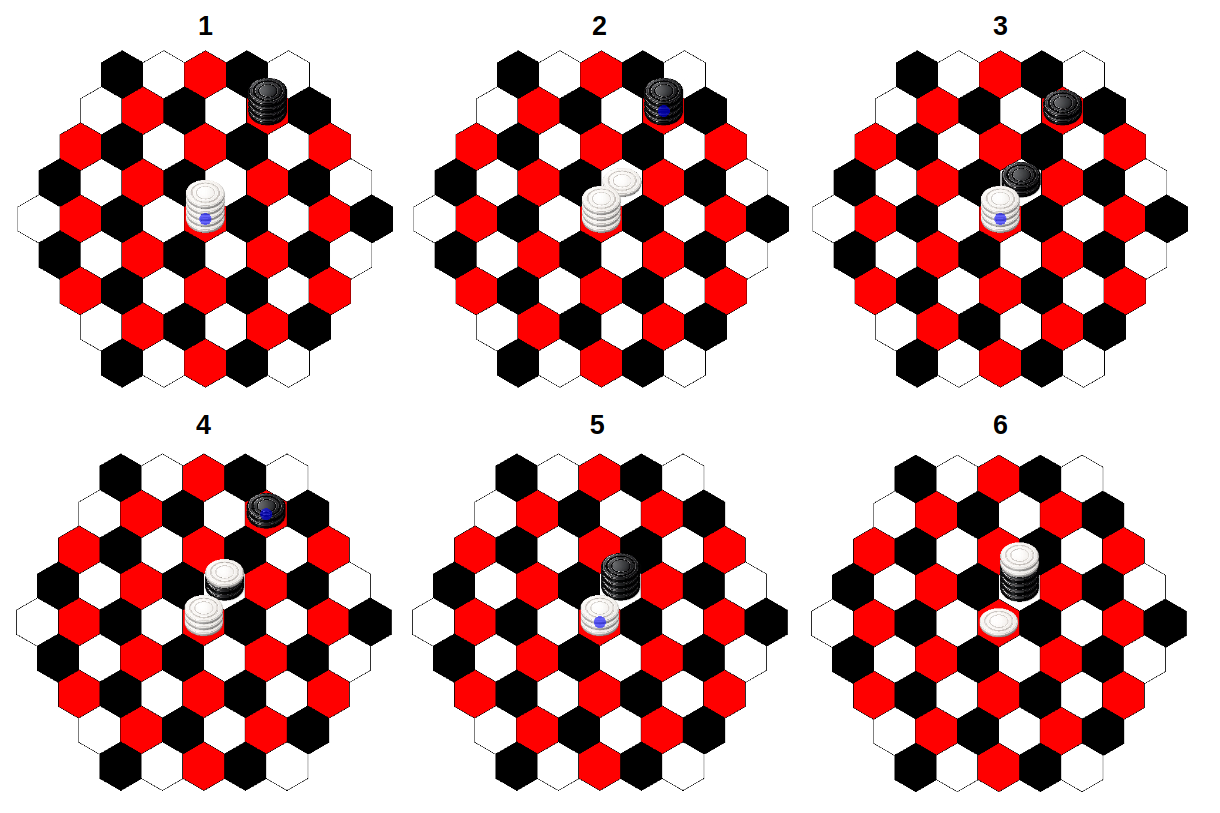
\includegraphics[scale=0.3]{advanced_ai_agents/images/diverse_figures/single_pawn_baiting.png}
    \caption{Figure displaying how the \textit{single-piece baiting} strategy used by the white player defeats the powerful stack of the black player.}
    \label{fig:single_pawn_baiting}
\end{figure}

This scenario illustrates how Player 1 forces Player 2 to dislocate their stack onto a white tile by moving a single piece at each turn. Since Player 2 is located further from the white tile, they are required to dislocate at least two pieces per turn. In the long run, this leads to Player 2 losing more pieces than Player 1, resulting in a win for Player 1.\footnote{After the final move, Player 1 still has one piece remaining on the initial tile, indicating that this strategy also applies when both players start with the same number of pieces on the initial tiles.}

An important question that arises is whether a smaller stack can defeat a larger stack using a \textit{single-piece baiting} attack.

In the following paragraph, it will be shown that the answer to this question is negative.\\

\textbf{Proof}:\\

First, it is important to specify that only scenarios in which both players have stacks on red tiles are relevant. This is because strong players typically aim to place their stacks onto red tiles as quickly as possible. Furthermore, we restrict our attention to positions in which the bait tile is white. Using a black or red tile as bait would advantage the defender by providing a more strongly supported stack, thereby forcing the attacker to commit additional pieces in order to sustain the attack.

From the geometry of the board, it can be observed that for any given tile, all tiles at distance three share the same color, as shown in~\ref{fig:all_tiles_are_red_at_dist_3}. This implies that a stack on a red tile cannot be attacked using a \textit{single-piece baiting} strategy with a bait tile located at distance three from the defender. In the most favorable case for the attacker, the white bait tile is located at distance two from the defender, as illustrated in the previous example~\ref{fig:single_pawn_baiting}.

\begin{figure}[h]
    \centering
    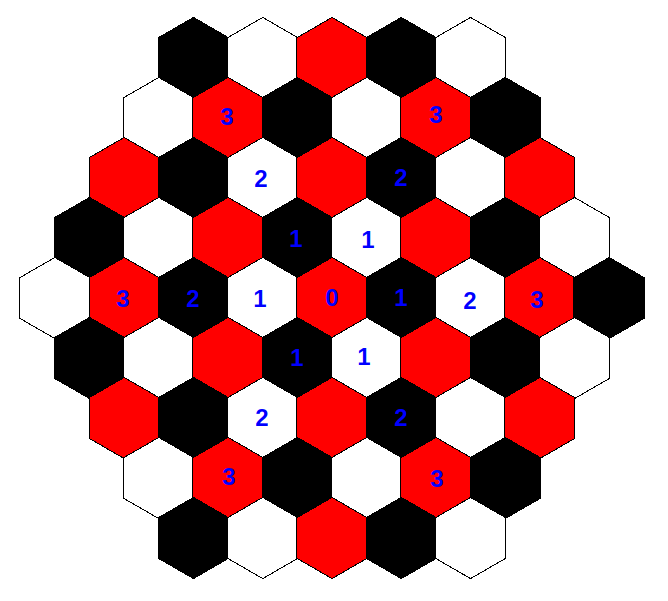
\includegraphics[scale=0.3]{advanced_ai_agents/images/diverse_figures/all_tiles_are_red_at_dist_3.png}
    \caption{Figure showing that all the tiles at distance 3 of the central red tile are also red.}
    \label{fig:all_tiles_are_red_at_dist_3}
\end{figure}

Now that the relevant scenarios for the single-piece baiting strategy have been established, we show that if the attacker has fewer pieces than the defender, the attack can never succeed. The flowchart in~\ref{fig:schema_single_pawn_bait} supports this claim by enumerating all possible moves available to the attacker.

\begin{figure}[h]
    \centering
    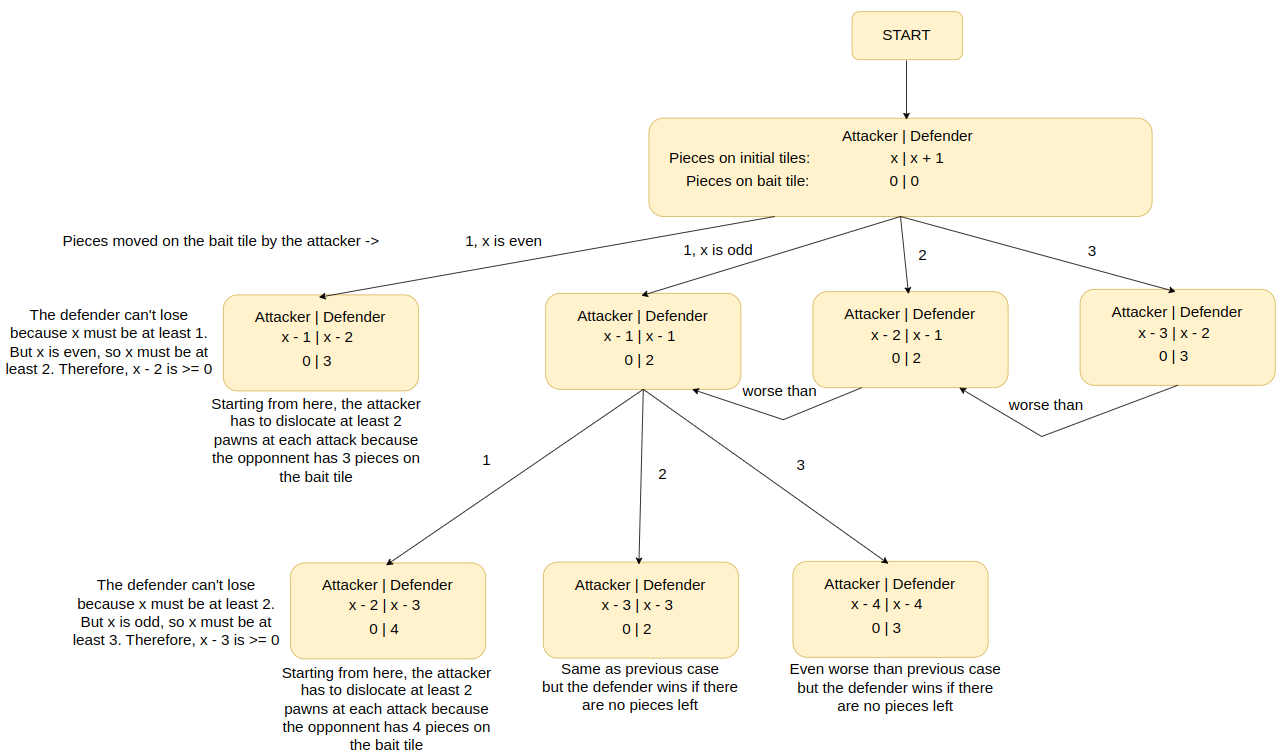
\includegraphics[scale=0.3]{strategic_analysis_and_heuristic_design/images/proof_schema_single_piece_baiting.png}
    \caption{Flowchart illustrating all possible move sequences during a \textit{single-piece baiting} attack.}
    \label{fig:schema_single_pawn_bait}
\end{figure}

Finally, this leads to the design of a third heuristic, which consists of prioritizing the concentration of pieces onto a minimal number of tiles. This is based on the observation that a small number of large stacks is preferable to a larger number of small stacks. As shown previously, a large stack on a red tile cannot be the victim of a \textit{single-piece baiting} attack from a smaller stack, whereas the opposite situation does not hold.

\section{Combined Heuristic and Limitations}

The heuristic evaluation used in this thesis combines the previous observations in a prioritized way. The first priority is the comparison of controlled material, since control of pieces directly affects mobility and the possibility of winning. The second priority is positional power, which rewards control of stronger tiles and more powerful stacks. Finally, the evaluation favors positions where pieces are grouped into stronger stacks rather than being spread across many weak stacks.

This prioritization is important. If positional power were weighted too strongly, an agent might sacrifice too many pieces only to occupy stronger tiles. Such behavior may improve the position locally, but it can be strategically poor if it reduces long-term control and mobility. Giving priority to material control helps avoid this problem.

The proposed heuristic remains handcrafted and therefore limited. It does not capture all tactical motifs of Tricolor, and its weights are not learned automatically from data. Moreover, some strategic features may only become visible through stronger self-play or deeper search. Nevertheless, the heuristic provides a useful first evaluation function for the Alpha-Beta agent introduced in the next chapter.

Future work could investigate automatic heuristic tuning or learning-based evaluation functions. This would be consistent with previous work on heuristic prediction in general game playing, where game descriptions are used to estimate which heuristic features are likely to perform well~\cite{stephenson2021heuristic}. In the case of Tricolor, such approaches could eventually help refine or replace the manually designed evaluation function.